%\documentclass[mathserif]{beamer}
\documentclass[handout]{beamer}
%\usetheme{Goettingen}
\usetheme{Warsaw}
%\usetheme{Singapore}
%\usetheme{Frankfurt}
%\usetheme{Copenhagen}
%\usetheme{Szeged}
%\usetheme{Montpellier}
%\usetheme{CambridgeUS}
%\usecolortheme{}
%\setbeamercovered{transparent}
\usepackage[english, activeacute]{babel}
\usepackage[utf8]{inputenc}
\usepackage{amsmath, amssymb}
\usepackage{dsfont}
\usepackage{graphics}
\usepackage{cases}
\usepackage{graphicx}
\usepackage{pgf}
\usepackage{epsfig}
\usepackage{amssymb}
\usepackage{multirow}	
\usepackage{amstext}
\usepackage[ruled,vlined,lined]{algorithm2e}
\usepackage{amsmath}
\usepackage{epic}
\usepackage{epsfig}
\usepackage{fontenc}
\usepackage{framed,color}
\usepackage{palatino, url, multicol}
\usepackage{listings}
%\algsetup{indent=2em}


\vspace{-0.5cm}
\title{Markov Chain Monte Carlo}
\vspace{-0.5cm}
\author[Felipe Bravo Márquez]{\footnotesize
%\author{\footnotesize  
 \textcolor[rgb]{0.00,0.00,1.00}{Felipe José Bravo Márquez}} 
\date{ \today }




\begin{document}
\begin{frame}
\titlepage


\end{frame}


%%%%%%%%%%%%%%%%%%%%%%%%%%%


\begin{frame}{Markov Chain Monte Carlo}
\scriptsize{
\begin{itemize}
\item This class  introduces estimation of posterior probability distributions using a stochastic process known
as \textbf{Markov chain Monte Carlo} (MCMC). 

\item Here we'll produce samples from the joint posterior without maximizing anything. 

\item We will be able to sample directly from the posterior without assuming a Gaussian, or any other, shape. 

\item The cost of this power is that it may take much longer for our estimation to complete.

\item But the benefit is escaping multivariate normality assumption of the Laplace approximation.

\item More advanced models such as the generalized linear and multilevel models tend produce non-Gaussian posterior distributions.

\item In most cases  they cannot
be estimated at all with the techniques of earlier classes. 


\item This class is based on Chapter 9 of \cite{mcelreath2020statistical} and Chapter 7 of \cite{kruschke2014doing}.
 
\end{itemize}



} 

\end{frame}




\begin{frame}{Markov Chain Monte Carlo}
\scriptsize{
\begin{itemize}
\item The essence of MCMC is to produce samples from the posterior $f(\theta|d)$ by only accessing a function that is proportial to it.
\item This proportial function is the product of the likelihood and the prior $f(d|\theta)*f(\theta)$, which is always available in a Bayesian model.
\item So, merely by evaluating $f(d|\theta)*f(\theta)$, without normalizing it by $f(d)$, MCMC allows us to generate random representative values from the posterior distribution.

\item This property is wonderful because the method obviates direct computation of the evidence $f(d)$, which, as you'll recall, is one of the most difficult aspects of Bayesian
inference. 

\item It has only been with the development of MCMC algorithms an software that Bayesian inference is applicable to complex data analysis.
\item And it has only been with the production of fast and cheap computer hardware that Bayesian inference is accessible to a wide audience.

\item The question then becomes this: How does MCMC work? For an answer, let's ask a politician. 
 
\end{itemize}



} 

\end{frame}




\begin{frame}{A politician stumbles upon the Metropolis algorithm}
\scriptsize{

\begin{itemize}
\item Suppose an elected politician lives on a long chain of islands.
\item He is constantly traveling from island to island, wanting to stay in the public eye. 
\item At the end of a day he has to decide whether to:

\begin{enumerate}
\scriptsize{
 \item stay on the current island
 \item move to the adjacent island to the west
 \item move to the adjacent island to east }
\end{enumerate}

\item His goal is to visit all the islands \textbf{proportionally} to their \textbf{relative population}.

\item But, he doesn't know the total population of all the islands.
\item He only knows the population of the current island where he is located.
\item He can also ask about the population of an adjacent island to which he plans to move.

\end{itemize}


} 
\end{frame}


\begin{frame}{The Metropolis algorithm}
\scriptsize{

\begin{itemize}
\item The politician has a simple heuristic for travelling accross the islands called the \textbf{Metropolis} algorithm \cite{metropolis1953equation}.

\item First, he flips a (fair) coin to decide whether to propose the adjacent island to the left or the adjacent island to the right.

\item If the proposed island has a larger population than
the current island ($P_{proposed}>P_{current}$), then he  goes to the proposed island.

\item If the proposed island has a smaller population than the current island ($P_{proposed}<P_{current}$), then he goes to the proposed island with probability $p_{move}=P_{proposed}/P_{current}$.


\item In the long run, the probability that the politician is on any one of the islands exactly matches the relative population of the island!

\end{itemize}


} 
\end{frame}


\begin{frame}{The Metropolis algorithm}
\scriptsize{

\begin{itemize}
\item Let's analyze the Metropolis algorithm in more detail.
\item Suppose there are 10 islands in total.
\item Each island is neighbored by two others, and the
entire archipelago forms a ring.
\item The islands are of different sizes, and so had different sized populations living on them.
\item The second island is twice as populous as the first,
the third three times as populous as the first.
\item And so on, up to the largest island, which is 10 times as populous as the smallest.

\end{itemize}


} 
\end{frame}


\begin{frame}{The Metropolis algorithm}

   \begin{figure}[h!]
	\centering
	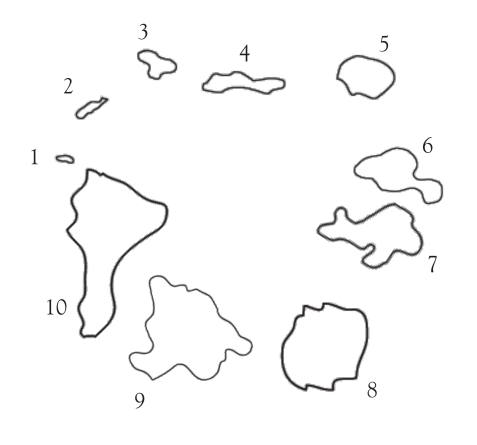
\includegraphics[scale=0.5]{pics/islands.png}
	\end{figure} 

\end{frame}




\begin{frame}{The Metropolis algorithm}
\scriptsize{

\begin{itemize}
\item We are going to show an implementation of this algorithm in R.

\item But before that, we will combine combine the two possibilities for the probability of moving into a single expression: the proposed island having a 1) higher or 2) lower population than the current island.

\begin{equation}
p_{move}=\min(1,P_{proposed}/P_{current}). 
\end{equation}

\item So, if $P_{proposed}>P_{current}$, $P_{proposed}/P_{current}>1$ and $p_{move}=1$.

\item For example, $current=4$ and $proposed=5$, $5/4>1$ so we move to the proposed island (with probability 1). 

\item On the other hand, if $P_{proposed}<P_{current}$, $P_{proposed}/P_{current}<1$, and $p_{move}=P_{proposed}/P_{current}$.

\item For example, $current=4$ and $proposed=3$, $3/4<1$ so we move to the proposed island with probability $3/4$.

\end{itemize}


} 
\end{frame}



\begin{frame}[fragile]{The Metropolis algorithm}
\scriptsize{


\begin{verbatim}
num_days <- 1e5
positions <- rep(0,num_days)
current <- 10
for ( i in 1:num_days ) {
  # record current position
  positions[i] <- current
  # flip coin to generate proposal
  proposal <- current + sample( c(-1,1) , size=1 )
  # now make sure he loops around the archipelago
  if ( proposal < 1 ) proposal <- 10
  if ( proposal > 10 ) proposal <- 1
  # move?
  prob_move <- min(proposal/current,1)
  decision <- rbinom(1,1,prob_move)
  current <- ifelse( decision == 1 , proposal , current )
}

library(rethinking)
simplehist(positions,xlab="island",ylab="number of days")
\end{verbatim}



} 
\end{frame}


\begin{frame}{The Metropolis algorithm}

   \begin{figure}[h!]
	\centering
	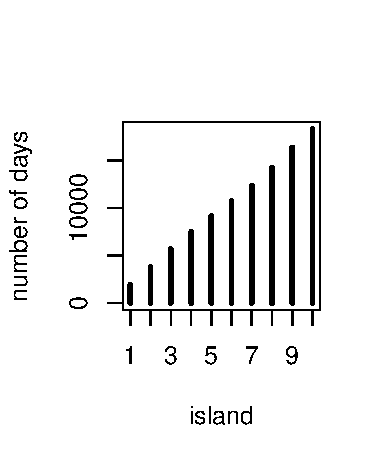
\includegraphics[scale=0.92]{pics/mcmc_islands.pdf}
	\end{figure} 

\scriptsize{
	The time spent on each island is proportional to its population size.}
	
\end{frame}



\begin{frame}{The Metropolis algorithm}
\scriptsize{

\begin{itemize}
\item The first three lines of the method just define
the number of days to simulate, an empty history vector, and a starting island position (the biggest island, number 10).
\item Then the for loop steps through the days. 
\item Each day, it records the politician's current position.
\item Then it simulates a coin flip to nominate a proposal island. 
\item The only trick here lies in making sure that a proposal of ``11'' loops around to island 1 and a proposal of “0” loops around to island 10.
\item Finally, a random binary number is generated with a binomial distribution with probability of success (or moving)$=\min(1,P_{proposed}/P_{current})$.
\item If this random number is 1 we move, otherwise we stay.

\end{itemize}


} 
\end{frame}




\begin{frame}{The Metropolis algorithm}
\scriptsize{

\begin{itemize}
\item In real applications, the goal is not to help a politician, but instead to draw samples from an unknown and usually complex posterior probability distribution.
\item The ``islands'' in our objective are parameter values $\theta$, and they need not be discrete, but can instead take on a continuous range of values as usual.
\item The ``population sizes'' in our objective are the posterior probabilities (or densities) at each parameter value: $f(\theta|d)$
\item The ``days'' in our objective are samples taken from the posterior distribution.

\item The Metropolis algorithm will eventually give us a collection of samples from the posterior. 

\item We can then use these samples just like all the samples we have already used in this course.

\end{itemize}


} 
\end{frame}



\begin{frame}{Why it works}
\scriptsize{

\begin{itemize}
\item Now, let's try to understand why the algorithm works.

\item Consider two adjacent positions and the probabilities of moving from one to the other. 
\item We'll see that the relative transition probabilities, between adjacent positions, exactly match the relative values of the target distribution.

\item Extrapolate that result across all the positions, and you can see that, in the long run, each position will be visited proportionally to its target value.

\item Suppose we are at position $\theta$. 

\item The probability of moving to $\theta+ 1$, denoted
$P(\theta \rightarrow \theta + 1)$, is the probability of proposing that move times the probability of
accepting it if proposed, which is:
\begin{displaymath}
P(\theta \rightarrow \theta + 1) = 0.5 \times \min(P(\theta+ 1)/P(\theta),1) 
\end{displaymath}



\end{itemize}


} 
\end{frame}



\begin{frame}{Why it works}
\scriptsize{

\begin{itemize}
\item On the other hand, if we are presently at position $\theta+ 1$, the probability of moving to $\theta$ is:
\begin{displaymath}
P(\theta+1 \rightarrow \theta) = 0.5 \times \min(P(\theta)/P(\theta+1),1) 
\end{displaymath}

\item The ratio of the transition probabilities is:

  \begin{figure}[h!]
	\centering
	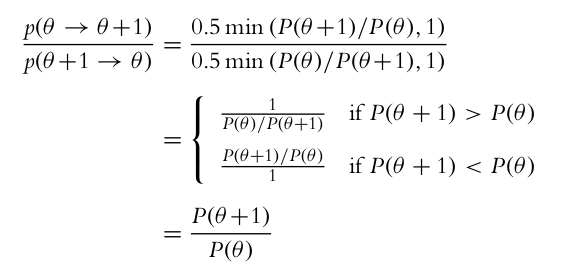
\includegraphics[scale=0.4]{pics/trans_ratio.png}
	\end{figure} 

\end{itemize}


} 
\end{frame}


\begin{frame}{Why it works}
\scriptsize{

\begin{itemize}
\item The last equation tells us that during transitions back and forth between adjacent positions, the relative probability of the transitions exactly matches the relative values of the target distribution. 
\item That might be enough to get the intuition that, in the
long run, adjacent positions will be visited proportionally to their relative values in the target distribution. 
\item If that's true for adjacent positions, then, by extrapolating from one position to the next, it must be true for the whole range of positions.

\item In more mathematical terms, this means that the transition probabilities form a Markov chain that has the target distribution as its equilibrium or stationary distribution. \cite{wiki:Markov_chain_Monte_Carlo}

\item Hence, one can obtain a sample of the desired distribution by recording states from the chain.


\end{itemize}


} 
\end{frame}


\begin{frame}{The Metropolis Algorithm more Generally}
\scriptsize{

\begin{itemize}
\item So far, we have only considered the case with a single discrete parameter $\theta$ that can only move to the left or right.

\item The general Metropolis algorithm allows working with multiple continuous parameters $\theta_1,\theta_2,\dots,\theta_n$ and more general proposal distributions.  


\item The essentials of the general method are the same as for the simple case. 

\item First, we have some target distribution $P(\theta)$ ($\theta$ can be a vector of parameters) from which we would like to generate representative sample values. 

\item We must be able to compute the value of $P(\theta)$ for any candidate value of $\theta$. 
\item The distribution, $P(\theta)$, does not have to be normalized, however. 

\item Just needs needs to be nonnegative. 


\end{itemize}


} 
\end{frame}


\begin{frame}{The Metropolis Algorithm more Generally}
\scriptsize{

\begin{itemize}

\item In our Bayesian inference application $P(\theta)$ is the unnormalized posterior distribution on  $\theta$, which is the product of the likelihood and the prior: $f(d|\theta)*f(\theta)$.

\item This is a very important property of MCMC, as it allows us to draw samples from the posterior without having to calculate the evidence $f(d)$.

\item Sample values from the target distribution are generated by taking a random walk through the parameter space.

\item Proposal distributions can take many different forms,  the goal being to use a proposal distribution
that efficiently explores the regions of the parameter space where $P(\theta)$ has most of its probability area. 

\item The generic case is using a Gaussian distribution  centered at the current position. 

\item So the proposed move will typically be near the current position, with the probability of proposing a more distant position dropping off according to the normal curve.

\item For multivariate target distributions, we can use a Multi-variate Gaussian to propose multi-dimensional points in each step. 


\end{itemize}


} 
\end{frame}


\begin{frame}{Gibbs Sampling}
\scriptsize{

\begin{itemize}

\item The Metropolis algorithm works whenever the probability of proposing a jump to B from A is equal to the probability of proposing A from B, when the proposal distribution is symmetric (such as a Gaussian distribution). 

\item There is a more general method, known as Metropolis-Hastings, that allows asymmetric proposals.

\item This would mean, that the politician's coin were biased to lead him clockwise on average.

\item Asymmetric proposal distributions allows us to explore the posterior distribution more efficiently (i.e., acquire
a good image of the posterior distribution in fewer steps).

\item Gibbs sampling is a variant of the Metropolis-Hastings algorithm that uses clever proposals and is therefore more efficient.

\item The improvement arises from adaptive proposals in which the distribution of proposed parameter values adjusts itself intelligently, depending upon the parameter values at the moment.


\end{itemize}


} 
\end{frame}


\begin{frame}{Gibbs Sampling}
\scriptsize{

\begin{itemize}

\item How Gibbs sampling computes these adaptive proposals depends upon using particular combinations of prior distributions and likelihoods known as conjugate pairs (such as Binomial and the Beta). 

\item Conjugate pairs have analytical solutions for the posterior distribution of an individual parameter. 

\item And these solutions are what allow Gibbs sampling to make smart jumps around the joint posterior distribution of all parameters.

\item The algorithm works as follows:

\item At each point in the walk, the parameters are selected in an iterative cycle: $\theta_1, \theta_2, \theta_3 , \dots \theta_1, \theta_2, \theta_3, \dots.$ 

\item Suppose that parameter $\theta_i$ has been selected.

\item Gibbs sampling then chooses a new value for that parameter by generating a random value directly from
the conditional probability distribution of that parameter given all the others and $d$: 

\begin{displaymath}
f(\theta_i | \theta_1,\dots, \theta_{i-1}, \theta_{i+1}, \dots,\theta_n,d)  
\end{displaymath}





\end{itemize}


} 
\end{frame}


\begin{frame}{Gibbs Sampling}
\scriptsize{

\begin{itemize}

\item As we are using conjugate pairs, this conditional probabilities distribution has a closed form and is easy to sample random numbers from it.

\item The new value for $\theta_i$ , combined with the unchanged values of $\theta_1,\dots, \theta_{i-1}, \theta_{i+1}, \dots,\theta_n$, constitutes the new position in the random walk.

\item The process then repeats: select the next parameter $\theta_{i+1}$ and select a new value for that parameter from its conditional posterior distribution.

\item Let's illustrate this process for a two-parameter example: $\theta_1,\theta_2$.

\item In the first step, we want to select a new value for $\theta_1$ . 

\item We conditionalize on the values of all the other
parameters from the previous step in the chain. 

\item In this example, there is only one other parameter, namely $\theta_2$.


\end{itemize}


} 
\end{frame}



\begin{frame}{Gibbs Sampling}
\scriptsize{


 \begin{figure}[h!]
	\centering
	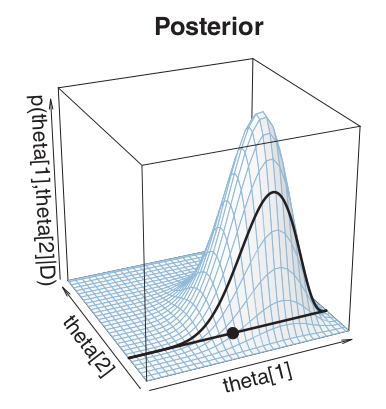
\includegraphics[scale=0.4]{pics/gibbs1.png}
	\end{figure} 

\begin{itemize}

\item The figure shows a slice through the joint distribution at the current value of $\theta_2$. 

\item The heavy curve is the posterior distribution conditional on this value of $\theta_2$, which is $f(\theta_1|\theta_2 , d)$ in this case because there is only one other parameter.

\end{itemize}


} 
\end{frame}


\begin{frame}{Gibbs Sampling}
\scriptsize{


\begin{itemize}

\item Because we are using conjugate pairs a computer can directly generate a random  value of $\theta_1$ from $f(\theta_1|\theta_2 , d)$. 

\item Having generated a new value for $\theta_1$, we then conditionalize on it and determine the conditional distribution of the next parameter, $\theta_2$ using $f(\theta_2|\theta_1 , d)$  as shown below:

 \begin{figure}[h!]
	\centering
	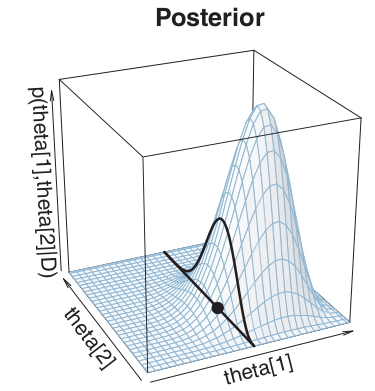
\includegraphics[scale=0.4]{pics/gibbs2.png}
	\end{figure} 

\item We generate a new value of $\theta_2$ , and the cycle repeats.



\end{itemize}


} 
\end{frame}


\begin{frame}{Gibbs Sampling}
\scriptsize{

\begin{itemize}

\item Because the proposal distribution exactly mirrors the posterior probability for that parameter, the proposed move is always accepted.

\item Hence, the algorithm is more efficient than the standard Metropolis algorithm in which proposals are rejected in many cases.

\item But there are some limitations to Gibbs sampling.

\item First, there are cases when we don't want to use conjugate priors. 

\item Second, it can become inefficient with complex models containing hundreds, thousands or tens of thousands of parameters.


\end{itemize}


} 
\end{frame}


\begin{frame}{Conclusions}
\scriptsize{

\begin{itemize}
\item Blabla
\end{itemize}


} 
\end{frame}


%%%%%%%%%%%%%%%%%%%%%%%%%%%
\begin{frame}[allowframebreaks]\scriptsize
\frametitle{References}
\bibliography{bio}
\bibliographystyle{apalike}
%\bibliographystyle{flexbib}
\end{frame}  









%%%%%%%%%%%%%%%%%%%%%%%%%%%

\end{document}
